\let\negmedspace\undefined
\let\negthickspace\undefined
\documentclass[journal]{IEEEtran}
\usepackage[a5paper, margin=10mm, onecolumn]{geometry}
\usepackage{lmodern} % Ensure lmodern is loaded for pdflatex
\usepackage{tfrupee} % Include tfrupee package

\setlength{\headheight}{1cm} % Set the height of the header box
\setlength{\headsep}{0mm}     % Set the distance between the header box and the top of the text

\usepackage{gvv-book}
\usepackage{gvv}
\usepackage{cite}
\usepackage{amsmath,amssymb,amsfonts,amsthm}
\usepackage{algorithmic}
\usepackage{graphicx}
\usepackage{textcomp}
\usepackage{xcolor}
\usepackage{txfonts}
\usepackage{listings}
\usepackage{enumitem}
\usepackage{mathtools}
\usepackage{gensymb}
\usepackage{comment}
\usepackage[breaklinks=true]{hyperref}
\usepackage{tkz-euclide} 
\usepackage{listings}                                      
\def\inputGnumericTable{}                                 
\usepackage[latin1]{inputenc}                                
\usepackage{color}                                            
\usepackage{array}                                            
\usepackage{longtable}
\usepackage{multicol}
\usepackage{calc}                                             
\usepackage{multirow}                                         
\usepackage{hhline}                                           
\usepackage{ifthen}                                           
\usepackage{lscape}
\begin{document}
	
	\bibliographystyle{IEEEtran}
	\vspace{3cm}
	
	\title{11.16.3.8.3}
	\author{EE24BTECH11047 - Niketh Prakash Achanta }
	{\let\newpage\relax\maketitle}
	
	\renewcommand{\thefigure}{\theenumi}
	\renewcommand{\thetable}{\theenumi}
	\setlength{\intextsep}{10pt} % Space between text and floats
	
	\numberwithin{equation}{enumi}
	\numberwithin{figure}{enumi}
	\renewcommand{\thetable}{\theenumi}
	
\textbf{Question}:\\
Three coins are tossed once. Find the probability of getting at least 2 heads.\\

\textbf{Solution: }\\

\textbf{Theoretical solution: }\\
To calculate the probability of getting at least 2 heads:

\begin{itemize}
    \item The total number of outcomes when three coins are tossed is:
    \[
    2^3 = 8
    \]
    \item The favorable outcomes for at least 2 heads are: \(HHT, HTH, THH, HHH\). Thus, there are 4 favorable outcomes.
    \item The probability of getting at least 2 heads is:
    \[
    P(\text{At least 2 heads}) = \frac{\text{Number of favorable outcomes}}{\text{Total outcomes}} = \frac{4}{8} = \frac{1}{2}.
    \]
\end{itemize}

Thus, the probability of getting at least 2 heads is:
\[
\boxed{\frac{1}{2}}
\]

\textbf{Computational solution: }\\

\section*{Z-Transform Computational Method for Coin Toss PMF}
\subsection*{PMF for a Single Coin Toss}
For a single coin toss, the probability mass function (PMF) is:
\[
P_X(x) =
\begin{cases}
p, & \text{if } x = 1 \text{ (Heads)} \\
1-p, & \text{if } x = 0 \text{ (Tails)}
\end{cases}
\]
where \(p = 0.5\) for a fair coin.

\subsection*{Z-Transform Expansion}
The Z-transform for the number of heads in \(n\) coin tosses is given by:
\begin{align}
H(z) = \left( p + (1-p)z \right)^n
\end{align}
where:
\begin{itemize}
    \item \(p = 0.5\), \(1-p = 0.5\),
    \item \(n = 3\).
\end{itemize}

\subsection*{Expansion of \(H(z)\)}
Expand the expression \(\left( p + (1-p)z \right)^n\) using the binomial theorem:
\begin{align}
H(z) = \sum_{k=0}^{n} \binom{n}{k} p^{n-k} (1-p)^k z^k
\end{align}

\subsection*{Result for \(n = 3\)}
Substituting \(n = 3\) and expanding:
\begin{align}
H(z) = (0.5 + 0.5z)^3 = 0.125 + 0.375z + 0.375z^2 + 0.125z^3
\end{align}

The PMF values for heads are:
\begin{align}
P_X(0) = 0.125, \quad P_X(1) = 0.375, \quad P_X(2) = 0.375, \quad P_X(3) = 0.125
\end{align}

The probability of getting at least 2 heads is:
\[
P_X(2) + P_X(3) = 0.375 + 0.125 = 0.5
\]

\section*{Conclusion}
The probability of getting at least 2 heads is:
\[
\boxed{0.5}
\]
	\begin{figure}[h!]
		\centering
		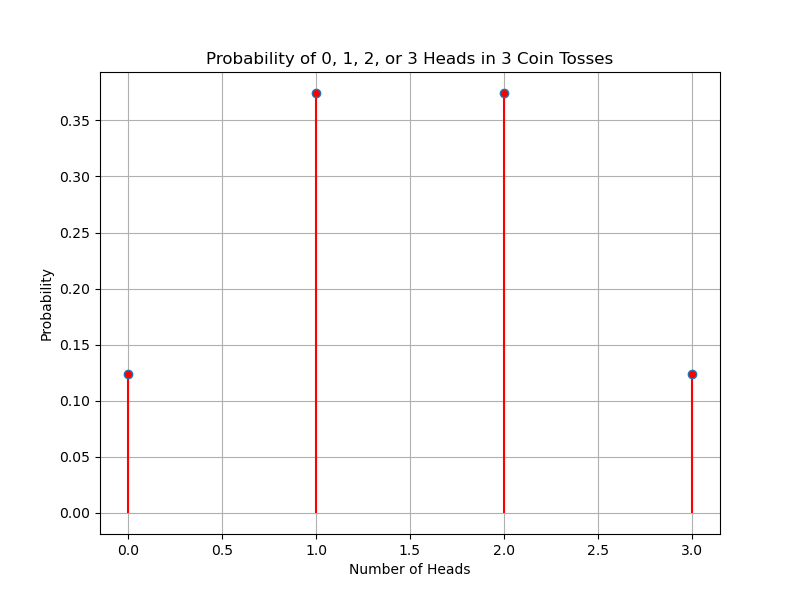
\includegraphics[width=\columnwidth]{/home/niketh/EE1003/3.8.3/figs/Figure_1.png}
		\label{stemplot}
	\end{figure}
\end{document}

